\documentclass[12pt]{article}
\usepackage[paper=a4paper, margin=1in]{geometry} 

%Required packages
\usepackage{natbib} 
\usepackage{graphicx}
\usepackage{amsmath}
\usepackage{mathtools}
\usepackage{setspace}
%\usepackage[document]{ragged2e}
\usepackage{lineno}
\usepackage{gensymb}
\setcounter{secnumdepth}{-1} 
%\raggedright
\title{ What controls the range of hosts a fish parasite infects?}
\author{Tad Dallas$^{1,2}$, Andrew Park $^{1}$, and John M. Drake$^{1}$}
\date{}

\begin{document}
\setcounter{page}{1}
\maketitle{}
\vspace{-0.5cm}

\begin{enumerate}
  \item University of Georgia, Odum School of Ecology, 140 E. Green Street, Athens GA, 30602. 
  \item Corresponding author: \texttt{tdallas@uga.edu}
\end{enumerate}

\linenumbers
\doublespacing

\section*{Abstract}





\section*{Keywords}
FishPEST, species distribution model, boosted regression tree, 



 
\section*{Introduction}

% Parasites may be really host specific, or generalist. This is controlled by a variety of factors, and makes predicting parasite species distributions among potential host species pretty difficult.  

Parasites are ubiquitous in nature, and are incredibly diverse in their life histories, transmission modes, and degree of host specificity \citep{poulin2011}. The question of what constrains which hosts a parasite infects is a central question to disease ecology. On one hand, host-parasite relationships may be viewed as complex interactions determined by environment \citep{locke2013}, geography \cite{nieberding2008}, co-evolutionary history \cite{krasnov2012}, or trait matching between host and parasite \cite{rohr2013}. On the other, host-parasite interactions may be viewed as random \cite{kennedy2009}, or neutral interactions, such that predicting which hosts a parasite will infect is either impossible, or determined simply based on host abundance \cite{canard2014}. The degree to which host-parasite interactions are environmentally constrained, and therefore predictable, is unclear. Previous efforts to characterize parasite communities have largely focused on parasite richness \citep{arneberg2002,nunn2003,ezenwa2006,poulin1997} instead of parasite community composition. Further, studies examining parasite community composition have focused efforts on topological measures of host-parasite networks \citep{guegan1994, canard2014, krasnov2012, poulin2010} or examined distance decay relationships in parasite community dissimilarity \citep{locke2012, locke2013, poulin2003}. The ability to 1) discern if host-parasite interactions are simply neutral processes, and 2) predict the identity of the subset of hosts able to be infected by a particular parasite is a large knowledge gap in the study of parasite ecology. From an applied perspective, parasite host range prediction could be useful for forecasting potential parasite spillover events to novel hosts \cite{colautti2004}, including humans \cite{daszak2000}. \\


%This presents an interesting prediction problem, where it may be possible to predict which hosts a parasite will infect. What does this problem require? What determines what hosts a parasite will infect?

One of the largest factors holding predictive models of parasite distributions among potential hosts is the relative paucity of data (but see \cite{}). However, this barrier is being overcome both by scientists \cite{strona2012, nunn2005} and museums (\cite{gibson2005}). Studies utilizing these large datasets have largely asked questions about parasite co-occurrence patterns \cite{strona2013}, or the factors influencing parasite sharing \cite{braga2014, dallas2014b}. These studies largely examine parasite community composition, and determine the influence of host traits or phylogenetic relationships on parasite community composition. However, few studies have attempted to predict which hosts a given parasite species will infect, despite the importance of this question to public health, and host-parasite network structure. Specifically, efforts predicting parasite spillover to humans may be essential for mitigation of zoonotic diseases. Further, the ability to predict which hosts an introduced parasite will infect in the native community can guide management decisions, and effectively predict change in host-parasite network structure. Previous efforts to predict parasite species host ranges have been hampered by the use of deprecated niche modeling algorithms, and conceptual differences in study goals \citep{strona2012}. Specifically, \citet{strona2012} developed a framework, specifically \texttt{PaNic} \citep{strona2012panic}, that estimates parasite niche boundaries as defined by the host traits of known hosts, and then estimated which hosts \textit{could} become parasitized by the given parasite species, given constraints (e.g., host family, geographic location) imposed by the user. Our goal is slightly different from this, in that we aimed to develop predictive, validated models that would allow for the determination of the relative importance of host traits, geographic variables, and other parasites that infect a given host species. This aim addresses a central gap in our understanding of host specificity in parasites; what constrains which hosts get infected by a given parasite species? \\ 
 
   
%\paragraph{Thesis}
 We address this knowledge gap by using a large database on freshwater fish prasites \citep{strona2013}, in order to develop predictive parasite species distribution models for a number of parasite species. In doing so, we can address the predictive capability of models trained on different variable classes. Parasite occurrence is likely not a simple function of host traits, as previous modeling efforts have assumed. Specifically, the number and identity of host species that a given parasite could infect may be constrained by geographic location, host trait variables (i.e. patch quality), or the existing parasite community of the given host species (i.e. parasite community structure). To address the relative importance of these variable classes, we trained boosted regression models on each of these three variable classes, and compared the accuracy obtained from each model in predicting the potential distributions of 238 parasite species. Parasite species distributions were most constrained by the existing parasite community, as this model allowed for highly accurate prediction of parasite occurrence likelihood. Models trained on host traits had poor predictive capabilities, and models trained on geographic variables had intermediate predictive accuracy. Taken together, our findings suggest that predicting the host distribution of a given parasite species requires information on the parasite communities of the potential hosts, and not necessarily any information on host traits. 
  
 
%What constrains the range of hosts that a parasite can infect? Is there a simple range of host functional traits that can determine the likelihood that a parasite infects a given host species? How well can we predict parasite occurrences given \textit{only} host life history traits? How about using solely information on parasite community structure? 

%Does the importance of different host functional traits or parasite community information differ with parasite type? (supplement)


 
\section*{Methods}
 \paragraph{Data and processing}
  We use an existing global database of fish-parasite associations (hereafter referred to as FishPest; \citep{strona2013}) consisting of over 38,000 helminth parasite records spanning a large diversity of parasites (Acanthocephala, Cestoda, Monogenea, Nematoda, Trematoda). Many of these entries represent isolated occurrences of parasites on hosts. In order to allow for cross-validation and accurate prediction, we constrained our ananlyses to parasites with a minimum of 20 host records. In other words, we only examined parasites that had been recorded more than 20 times, but these occurrences could be on fewer than 20 host species. The inclusion of duplicate occurrences was only permitted if the parasite was recorded on a host in a different geographic location, based on latitude and longitude values. This resulted in a total of 238 parasite species. Our response variable was parasite occurrence (binary), and was predicted using three classes of variables, representing host life history traits, geographic location, and parasite community similarity (Table 1). \\
  
  Values of predictor variables were obtained largely through the FishPest database \cite{strona2012, strona2013}, supplemented by variables obtained from FishBase \cite{froese2010}. However, there were still some missing predictor variable values. Missing predictor variable values were imputed using the imputation procedure in the \texttt{randomForest} \texttt{R} package (\cite{randomForest}). Details of host trait and geographic variable determination are provided in \cite{strona2013} and Table \ref{tab:traits}. Parasite community structure was considered as the first five principal components from a principal components analysis on the host-parasite matrix. This matrix contains information on all parasites infecting all host species, except with the parasite species of interest removed. Thus, the principal components represent a measure of parasite community structure among host species without any information about host range of the parasite species under consideration. Typically, the cumulative proportion of variance explained from the first five principal components was low, with a mean value of 0.28 cumulative proportion of variance explained. In addition, we included parasite species richness of a host as a predictor variable, as this may reflect the susceptibility of host species to parasitism.    
  
 
 \paragraph{Predictive model formulation}
  Here, we used boosted regression trees to predict parasite occurrence among potential host species for each of our 238 parasite species. Regression tree analysis is an extremely powerful tool for prediction and feature selection, bypassing many of the issues of simple regression models (e.g. multicollinearity, nonlinear relationships) \cite{elith2008, dallas2014}. “Boosting” refers to the process of creating a large number of regression trees, and weighting them by their predictive power to extract general “weak” rules, which are then combined to enhance predictive ability. The optimal number of trees was determined using the out-of-bag (\texttt{OOB}) estimation procedure, with the upper limit set to 50000. Other pertinent parameters include the learning rate ($l$ = 0.001), which controls the degree each new tree contributes to the overall model, and interaction depth ($id$ = 4), which allows for up to four-way interactions among predictor variables. \\
  
  The absence of a recorded interaction between host and parasite does not mean that the parasite does not infect that host. Borrowing from the idea behind Maximum Entropy modeling, we sampled the data to obtain background interactions, which we define here as a set of possible interactions between host and parasites. This background set was not composed of the entire dataset, but rather a sample of five times the number of positive occurrence records for a given parasite. These data were subset into a training set, 70\% of the data used to train the boosted regression tree model, and a test set, the remaining 30\% of the data used to test the predictive accuracy of the trained model. \\
  
  From the final boosted regression tree models, we are able to extract variable relative contribution ($RC$) measures, which provide information about the importance of each variable to the final model predictions. Relative contribution values for each predictor variable was determined by permuting each predictor variable and quantifying the reduction in model performance, a method that is free of classical assumptions about normality and equal variance (Anderson 2001). Relative contribution estimates were then based on the number of times a given predictor variable was selected for splitting, weighted by the degree the split improves model performance, and scaled between 0 (no contribution) to 100 (maximum contribution). \\
  
  All models were compared to a random null model, which randomized occurrence values in the test dataset, but kept them constrained to the total number of occurrences. Model performance was assessed using receiver operating characteristic curves, which relate true positive and false positive (type I error) rates graphically. The area between the curve generated by true and false positives and the 1:1 line from the origin gives a measure of predictive accuracy. 
  
   
\section*{Results}

  \paragraph{Importance of host traits, geographic variables, and parasite community similarity}
  All models performed better than our null predictions (null model $\overline{AUC}$ = 0.50). With varying degrees of accuracy, models were able to predict parasite occurrence for the 238 parasite species examined using host traits ($\overline{AUC}$ = 0.66), geographic variables ($\overline{AUC}$ = 0.79), and parasite community similarity ($\overline{AUC}$ = 0.88). The full model containing all variables was able to successfully predict parasite occurrences in the hold-out test dataset with high accuracy ($\overline{AUC}$ = 0.89), only marginally more accurate than the model trained with only parasite community similarity variables (Figure \ref{fig:brtAccuracy}). The relative contribution ($RC$) values for each separate model, and the model trained on all available data are provided in Figure \ref{fig:megaBRT}.  \\
  
  In the full model, variables of different classes were allowed to have different relative contributions, which allows for the determination of variables driving the predictive accuracy of the full model. For instance, relative contribution values were largest for the parasite community similarity values obtained from the principal components analysis on the host-parasite network with the parasite species of interest removed (Figure \ref{fig:megaBRT}), with the five PCA vectors comprising around 52\% of the relative contribution values, and four of the top five predictive variables. On the other side of the predictive spectrum, host trait variables, specifically host age at maturity, lifespan, and growth rate, contributed very little to model performance. \\
    
  
  \paragraph{Was predictive ability influence by parasite ecology?} 
  
  The relative importance of variable classes, or the general predictive power of the trained model, may differ as a function of parasite taxonomic group or host specificity. We tested for variation in predictive power among parasite taxonomic group (Acanthocephalans, Cestodes, Monogeneans, Nematodes, and Trematodes) and as a function of the number of host specificity. Here, we defined parasite host specificity as the number of hosts a parasite infects. We failed to detect evidence that parasite taxonomic group (Figure S1) influenced predictive power in any of our trained models. We did, however, observe an effect of host specificity (Figure S2), as predictive accuracy became more variable as host specificity increased (i.e. the number of hosts a given parasite infected became smaller). Despite this variability, the the mean predictive accuracy over a range of host specificity values remained constant (Figure S2).  
  
  
  
\section*{Discussion}

 We provide evidence that host traits are not as important to determining which hosts a given parasite will infect relative to geographic location, or parasite community similarity. This suggests two things. First, the current paradigm that attempts to define a parasite's niche based on qualities of the host (e.g. body size) may need to be reconsidered. Second, it suggests that the parasite community infecting a given host species contains information that can either predict or preclude the occurrence of a novel parasite species on that host. Further, model predictive accuracy did not vary strongly as a function of parasite type or specificity, suggesting that our findings may be broadly applicable to parasites of different transmission modes, life histories, and degrees of specificity. Taken together, our analyses suggest that parasite communities of freshwater fish are not simply random assemblages, but are predictable with high accuracy given only information on coinfecting parasites. Further, our findings have implications to host community invasibility by novel parasites, parasite spillover, and host-parasite network structure. \\
 
  
 We found that host traits generally poorly predicted parasite occurrences, a striking finding given that a parasite's niche is often defined using information on host life history and phylogeny \citep{strona2012, rohde1993}. It is possible that host traits are important in structuring a parasite niche, especially host traits related to the ability of a parasite to infect a given host species (e.g. immune defenses, diet breadth, or geographic range) \citep{johnson2012}. This would be the case if the host traits measured here were not the traits that most constrain parasite occurrences, and if geographic and parasite community variables were highly correlated with unmeasured host traits. However, host traits examined here should have captured at least some information related to likelihood of parasite infection. Specifically, host population growth rate and host age at maturity are likely related to immune defenses \citep{zuk2002}, as host trophic level is related to exposure \citep{price1990}. Geographic variables predicted parasite occurrences more accurately, but the importance of individual geographic variables varied greatly among parasite species (Figure \ref{fig:megaBRT}), suggesting either that parasite species are responding to different geographic variables, or that a methodological aspect of the analysis causes no single variable to dominate predictions. This could occur if geographic variables were highly correlated, or if interactions among variables were very important (i.e. the interaction between latitude or longitude with geographic region). 
 
   
 Parasites may be introduced with the addition of non-native host species to communities. The successful integration of the non-native host may be either enhanced if parasites of the non-native host ``spillover'' to the resident host community, or reduced by the sharing of parasites from the resident host community to the potential invader (the so-called biotic resistance hypothesis; \citet{britton2013}). The ability to predict the likelihood of both avenues of parasite sharing could allow for the prediction of invasion probability based on the parasite community of host species present. Based on our work, predicting what resident host species are likely to become infected by a novel parasite requires only information on the parasite communities of the resident host species. This means that pre-invasion prediction of parasite spillover may be possible.  
 
  
  
  
  
  
  
\section*{Acknowledgements}

The Macroecology of Infectious Disease Research Coordination Network (funded by NSF DEB 131223) provided useful discussions and support for this work. TD, AP, and JMD were supported by the Odum School of Ecology at the University of Georgia.



\bibliographystyle{amnat}
\bibliography{carp.bib}


\newpage
\section*{Tables}
  \begin{table}[!h]
  \caption{Description and units of variables used to predict parasite occurrences.}
  \vspace{0.1cm}
  \begin{tabular}{cccc}
\hline
\textbf{Variable} &   \textbf{Units} &   \textbf{Description} &   \textbf{Range} \\ 
\hline
Age at maturity & years        & Age at sexual maturity  & 0.1 -- 34  \\ 
Growth rate     & years$^{-1}$ & Rate to approach asymptotic length & 0.02 -- 9.87 \\ 
Life span       & years        & Estimated maximum age & 0 -- 145  \\ 
Max length      & cm           & Maximum fish species length  & 1 -- 2000 \\ 
Trophic level   & --           & 1 + mean trophic level of food  &  2 -- 5\\ 
 & & &  \\
Area of occupancy   & No. 1x1 $\degree$ cells &  Global host distribution  & 1 -- 1610    \\
Geographic region   & --       &   Biogegraphic region        & -- \\ 
Latitude            & $\lvert$max - min$\rvert$ degrees & Latitudinal distribution         & 1 -- 148 \\ 
Longitude           & $\lvert$max - min$\rvert$ degrees & Longitudinal distribution        & 1 -- 359 \\ 
 & & &  \\
Parasite species richness & \# & No. parasite species of host species &  0 -- 89 \\
Principal components     &  -- & PCA axes of host-parasite network   & -11.7 -- 9.8 \\
\hline
  \end{tabular}
  \label{tab:traits}
\end{table}


   
   
   

\newpage
\section{Figures}
\begin{figure}[h!]
  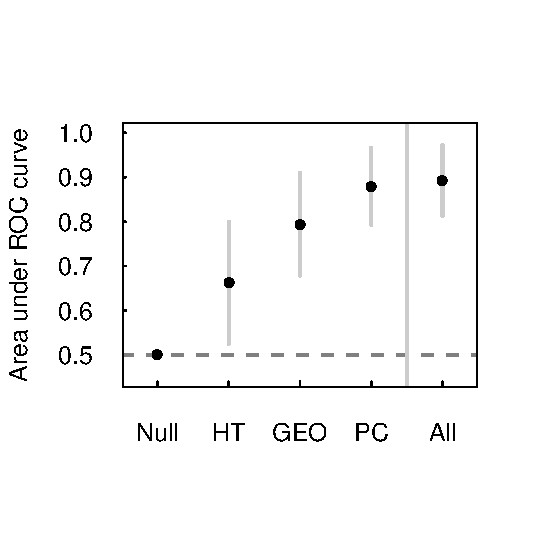
\includegraphics[width=\textwidth]{Figures/brtAccuracy.pdf}
  \caption{Accuracy, measured as the Area under Receiver operating characteristic (ROC) curves, for our predictive boosted regression tree models incorporating host traits (\texttt{HT}), geographic variables (\texttt{GEO}), parasite community information (\texttt{PC}), and the full model (\texttt{ALL}). These trained models were compared to a null model (\texttt{Null}) that maintained interaction number (number of occurrence records), but assigned occurrences equiprobably among potential interactors.}
 \label{fig:brtAccuracy}
 \end{figure}

 

 
\newpage
 \begin{figure}[h!]
  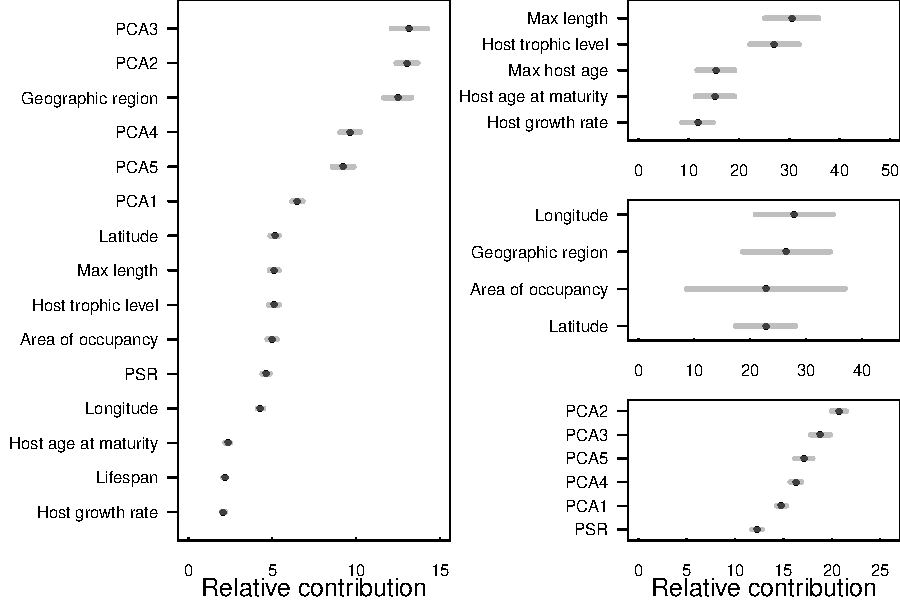
\includegraphics[width=\textwidth]{Figures/megaBRT.pdf}
  \caption{The average relative contribution values from the boosted regression tree models trained on all available data (left), host trait data (top right), geographic variables (middle right), and parasite community similarity (bottom right). Variables named ``PCA'' are principal components axes, and ``PSR'' refers to parasite species richness. Other variable definitions and units are available in Table 1. }
 \label{fig:megaBRT}
 \end{figure}

 
 
 \newpage
 \begin{figure}[h!]
  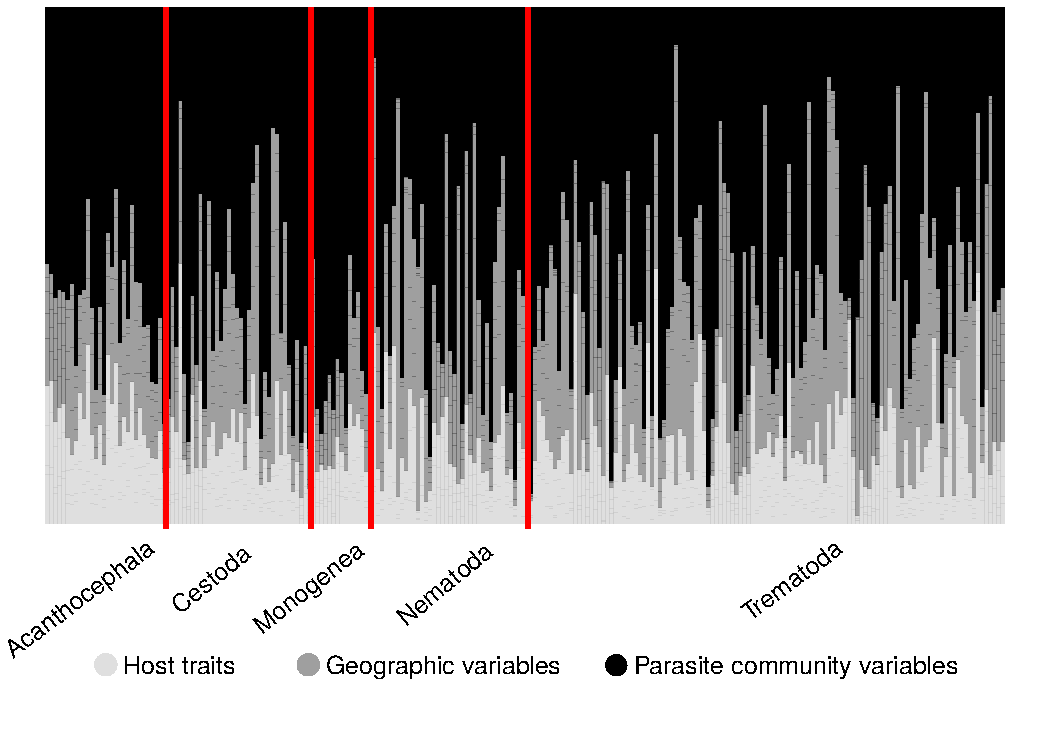
\includegraphics[width=\textwidth]{Figures/allDataColorGS1.pdf}
  \caption{Relative contribution values for variables of one of three classes; host traits, geographic variables, or parasite community variables. Each column represents a model trained on occurrence data for a single parasite species.}
 \label{fig:allDataBar}
 \end{figure}


 
 

%%%% Junk %%%%

%Predicting the distribution of a parasite species is challenging, because parasite occurrence requires passing through two filters. Assuming that the parasite is obligate at some point in its life cycle, the availability of competent hosts is the first filter, as the parasite will not be able to survive without a suitable host. Secondly, the parasite needs to be able to survive the environmental conditions of the area, so the environmental tolerances of the parasite represent the second filter. 

% SDMs of free-living species allow for prediction, and have applied use. Predicting what host species a parasite will infect is an obvious extension of SDM work, but it hasn't been done.
 %Species distribution modeling aims to predict the likelihood of species occurrence at a given location \citep{elith2009}, with obvious applications to monitoring threatened populations, predicting range expansion/contraction in changing environments \citep{guisan2005}, and assessing the risk of geographic locations to invasion from a non-native species. Only recently have these techniques been applied to modeling the suitability of geographic locations to parasite species \citep{giles2014, cornuault2013}. 
 %The complexity of host-parasite interactions limits our ability to predict what host species a parasite will infect
 
 
 




\end{document}
-